\documentclass[usenames,dvipsnames,letterpaper,landscape,final]{slides}

\def\fileHome{.}
\def\icons{\fileHome/icons}

\input mySlideStyle2019-1.tex
\def\myfboxBlack#1{\fboxrule2pt\fbox{$\ds#1$}}
\newcommand\topSeparatorHeading[1]{\noPagetrue\begin{myslide}\headingline\vbox to5.5in{%
\vfil\begin{center}{{\large\myfboxBlack{\myfboxBlack{%
\text{\ \ \bf\Blue{\begin{tabular}{c}#1\end{tabular}\ \ }}}}}}%
\end{center}\vfil}\end{myslide}\noPagefalse}

\usepackage{multirow}
\usepackage{enumitem}
\usepackage[ruled,vlined]{algorithm2e}
%\usepackage{wallpaper}
		  \usepackage{mathtools}
		  \usepackage{amsmath,amsthm,amsfonts,amscd}

\newcounter{outlineNumber}\setcounter{outlineNumber}{0}
\def\outno{\stepcounter{outlineNumber}\Blue{\theoutlineNumber. }}

\definecolor{boxColor}{rgb}{.4, .05, .2}

%------------------------------------------------------------------------------
\tikzset{cross/.style={cross out, draw=black, minimum size=2*(#1-\pgflinewidth), inner sep=0pt, outer sep=0pt},cross/.default={1pt}}

\renewcommand\floatpagefraction{0}
\renewcommand\textfraction{0}
\renewcommand\topfraction{1}
\renewcommand\bottomfraction{1}
\setcounter{topnumber}{10}
\setcounter{bottomnumber}{10}
\setcounter{totalnumber}{10}

\newtheorem{thm}{Theorem}
\newtheorem*{thm*}{Theorem}
\newtheorem{cor}[thm]{Corollary}
\newtheorem{lem}[thm]{Lemma}
\newtheorem*{lem*}{Lemma}
\newtheorem{prop}[thm]{Proposition}
\newtheorem{ax}{Axiom}

\theoremstyle{definition}
\newtheorem{defn}{Definition}

\newcommand{\commentedbox}[2]{%
  \mbox{
    \begin{tabular}[t]{@{}c@{}}
    $\boxed{\displaystyle#1}$\\
    #2
    \end{tabular}%
  }%
}

\newcommand{\Arrow}[1]{%
\parbox{#1}{\tikz{\draw[->](0,0)--(#1,0);}}
}

\def\picWidth#1#2{\includegraphics[clip=true,keepaspectratio=true,width=#1]{#2}}
\def\picHeight#1#2{\includegraphics[clip=true,keepaspectratio=true,height=#1]{#2}}
\def\picWidthHeight#1#2#3{\includegraphics[clip=true,width=#1,height=#2]{#3}}

 % =====================================
\def\d{\partial}
\def\grad{\nabla}
\def\div{\nabla\cdot}
\def\Div{\text{\rm div}}
\def\<{\langle}
\def\>{\rangle}

\let\vv=\v
%\def\G{\mathbf{G}}
\def\u{\mathbf{u}}
\def\U{\mathbf{U}}
\def\v{\mathbf{v}}
\def\V{\mathbf{V}}
\def\bpsi{\pmb{\psi}}
\def\bPsi{\pmb{\Psi}}
\def\bsigma{\pmb{\sigma}}
\def\bbV{{\mathbb{V}}}
\def\bbW{{\mathbb{W}}}

\def\cE{{\cal E}}
\def\cO{{\cal O}}
\def\cP{{\cal P}}
\def\cT{{\cal T}}

\def\D{\text{\rm D}}

\def\Po{\mathbb P}
\def\Re{\mathbb R}
\def\V{{\mathbb V}}
\def\W{{\mathbb W}}
\def\X{{\mathbb X}}

\def\cD{\mathcal{D}}
\def\cE{\mathcal{E}}
\def\cF{\mathcal{F}}
\def\cN{\mathcal{N}}
\def\cP{\mathcal{P}}
\def\cT{\mathcal{T}}

\def\RT{{\rm RT}}
\def\BR{{\rm BR}}
\def\St{{\rm S}}
\def\TH{{\rm TH}}
\def\J{{\text{\rm J}}}

\def\smallTwoVec(#1,#2){\Big(\begin{matrix}#1\\#2\end{matrix}\Big)}


\begin{document}

\begin{myslide}

\includegraphics[width=26cm,height=15cm]{intro.png}
\end{myslide}

\begin{myslide}
%          \heading{Motivation}
          \parbox{0.6\textwidth}{\raggedright
          %\subhead{Partial Melting in the Asthenosphere.}
          %\begin{blist}
          \Oorange{Partial melting} in the asthenosphere is a crucial geophysical process in lithospheric evolution and plate tectonics.
          %\item Determines the large-scale chemical evolution of the Earth.
          %\item Similar process may occur on extraterrestrial planets.
          %\end{blist}
          }\parbox{0.4\textwidth}{\raggedright
          \begin{center}
               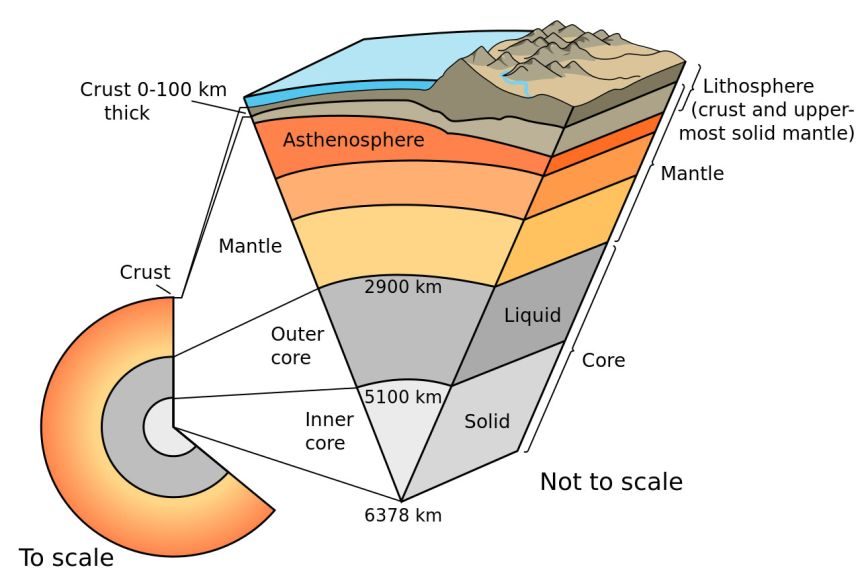
\includegraphics[width=9cm,height=7cm]{pics/cutaway-earth.jpg}
          \end{center} 
			 \qquad\tiny{(National Geographic)}
          }
         
\bigskip
\subhead{Goal.} Provide an \Oblue{accurate numerical approximation} of the time-dependent dynamics of a partially molten mantle.  

          \bigskip
          \subhead{Objective.}
          \begin{blist}
			 \item Provide a \Oblue{locally mass conservative} numerical framework for
						\begin{nlist}
          \item The mechanics of a deformable solid matrix that is possibly partially molten.
          \item The transport phenomena of chemical species and energy in the presence of
porous media.
						\end{nlist}
\item Connect static mechanical behavior and transport phenomena with proper phase behavior.
          \end{blist}
        %  \item Perform numerical simulation increase understanding of the physics.
          
\end{myslide}

\begin{myslide}
\heading{McKenzie Equations}
		  \begin{center}
					 \OliveGreen{\small(McKenzie 1984)}
		  \end{center}
\subhead{A two-phase formulation of a viscous mantle.}
\begin{equation*}
\begin{alignedat}{3}
		  &\phi_l (\mathbf{v}_l - \mathbf{v}_s)
		  + \frac{k_{\phi_l}}{\mu_l}(\nabla p_l - \rho_f\mathbf{g})
	    &&= 0, \qquad &&\Maroon{\text{(Darcy)}}\\
%		  &\nabla \cdot (\phi_l\mathbf{v}_l + \phi_s\mathbf{v}_s) &&=0,\\
		  &\nabla\bar p - \nabla \cdot \pmb{\tau}(\mathbf{v}_s) + \overline{\rho}\mathbf{g}&&= 0, \qquad &&\Maroon{\text{(Stokes)}}\\
%		  &\mu_s\nabla \cdot \mathbf{v}_s - \phi_l(p_l - p_s) &&=0, 
&\frac{\partial \rho_l \phi}{\partial t} + \nabla\cdot (\rho_l \phi \mathbf{v}_l) &&= \Oorange{\Gamma}  \qquad && \\
&\frac{\partial \rho_s (1-\phi)}{\partial t} + \nabla\cdot (\rho_s (1-\phi) \mathbf{v}_s) &&= \Oorange{-\Gamma}  \qquad && 
\end{alignedat}
\end{equation*}
\Oblue{Deviatoric stress of mixture}
\begin{equation*}\label{eq:deviatoricstress}
		  \pmb{\tau}(\mathbf{v}_s)
		  = 2\mu_s\phi_s\big( \tfrac{1}{2}(\nabla \mathbf{v}_s + \nabla \mathbf{v}_s^T) - \tfrac{1}{3}\nabla \cdot \mathbf{v}_s \mathbf{I}\big)
\end{equation*}

\parbox{0.5\textwidth}{\raggedright
\subhead{Unknowns.} \\
\Oorange{Four} equations and \Oorange{five} unknowns.
\begin{blist}
\item Velocities $\mathbf{v}_l$ and $\mathbf{v}_s$.
\item Pressure $p_l$ and $p_s$.
\item Porosity $\phi$ / Melting source $\Gamma$.
\end{blist}
}\parbox{0.5\textwidth}{\raggedright
\subhead{Three parts.}
\begin{blist}
\item Static mechanic equations.
\item Transport of chemical species and energy.
\item Phase package or prescribed melting function.
\end{blist}
}

\end{myslide}



\end{document}
